\chapter{\system Evaluation}
\label{chap:lazarusevaluation}


\section{Evaluation of Replica Set Risk}
\label{sec:diversity}

This section evaluates how \system performs on the selection of dependable \replica configurations.
As discussed in Section~\ref{sec:replica}, we focus our experimental evaluation solely on the OS diversity.
% These play a crucial role in any IT system, and most of the \replica's code is the OS. 
% Thus, they present a high potential to become the most vulnerable part of a \replica.
% Hence, in the following experiments, we explore OS diversity among the replicas. 

In these experiments, we emulate live executions of the system by dividing the collected data into two periods:
(i) a \emph{learning phase} covering all vulnerability data between \emph{2010-1-1} and \emph{2017-9-29}, which is used to setup the \risk's algorithm; and (ii) an \emph{execution phase} composed of the period between \emph{2017-10-1} and \emph{2018-3-30}.
This last period is divided into three intervals of two months (OUT-NOV, DEC-JAN, and FEB-MAR), allowing for three independent tests.
%JAN-FEB, MAR-APR, and MAY-JUN
The goal is to create a knowledge base in the \emph{learning phase} that is used to assess \system choices during each interval of the \emph{execution phase}. 
A run starts on the first day of an interval and then progresses through each day of the interval until the end. Every day, we check if the currently executing replica set could be compromised by an attack exploring the vulnerabilities released on that day. 
We take the most pessimist approach, which is to say that we consider the system to be broken if a vulnerability comes out that affects at least two OSes that would be executing at that time.

Three additional strategies, inspired by previous works, were defined to be compared with \system (Section~\ref{sec:configurations}):

\begin{itemize}
\item \textbf{Equal:} all the replicas use the same randomly-selected OS during the whole execution. 
This strategy corresponds to the scenario where most past \gls{bft} systems have been implemented and evaluated (e.g.,~\cite{Kotla:2010,Aublin:2015,Behl:2015,Veronese:2013,Behl:2017,Liu:2016,Yin:2003,Amir:2011,Bessani:2014,Clement:2009b}). 
Here, compromising a replica would mean an opportunity to intrude the remaining ones.

\item \textbf{Static:} a configuration of $n$ different \glspl{os} is randomly selected, and there are no changes during the whole execution. 
This corresponds to a diverse \gls{bft} system without reconfigurations (e.g.,~\cite{Rodrigues:2001}).

\item \textbf{Random:} a configuration of $n$ \glspl{os} is randomly selected, and at the beginning of each day, a new \gls{os} is randomly picked to replace an existing one. 
This solution represents a system with proactive recovery and diversity, but with no informed strategy for choosing the next \configuration.

%\item \textbf{\system}, $n$ OSes are chosen based the algorithm described in Section~\ref{sec:measurerisk}. This algorithm decides when it is time to replace OSes, which OS is out and which OS is in.
\end{itemize}

The experiments consider a pool of 38 \gls{os} versions to be deployed on four replicas. 
At the beginning of the execution phase, the OSes are assumed to be fully patched.

%\begin{figure}[t]
%\begin{center}
%\includegraphics[width=\columnwidth]{figs/gnuplot/executions/execution.pdf}
%\caption{Compromised system runs over 2 month slots.}
%\label{fig:all_vulns}
%\end{center}
%\end{figure}



\subsection{Diversity vs Vulnerabilities}
We evaluate how each strategy can prevent the replicated system from being compromised. 
Each strategy is analyzed over $5000$ runs throughout the execution phase in two-month slots. 
Different runs are initiated with distinct random number generator seeds, resulting in potentially different \gls{os} selections over the time slot. 
On each day, we check if there is a vulnerability affecting more than one replica in the current \configuration, and in the affirmative case the execution is stopped.

\begin{figure}[h]
\begin{center}
\includegraphics[width=\columnwidth]{images/gnuplot/executions_new/execution.pdf}
\caption{Compromised system runs over 2 month slots.}
\label{fig:all_vulns}
\end{center}
\end{figure}

\textbf{Results:} Figure~\ref{fig:all_vulns} compares the percentage of compromised runs of all strategies. 
Each bar represents the percentage of runs that did not terminate successfully (lower is better). 
In all three periods, \system presents the best results. 
The \emph{Random} strategy performs worse because eventually, it picks a group of \glspl{os} with common vulnerabilities. 
This result provides evidence for the claim that \system improves the dependability, reducing the probability that $f+1$ \glspl{os} eventually become compromised. 
Interestingly, and contrary to intuition, changing \glspl{os} every day with no criteria will always create unsafe configurations.
Therefore, it is paramount to have selection strategies like the ones we use in \system.
\note{Add all the months we already have}

\subsection{Risk evaluation}


In order to better understand how \system performed, we isolated one of the $5000$ runs to observe the risk evolution over time. 
We picked the \emph{Random} and \system strategies for this analysis, with results displayed in Figure~\ref{fig:run_all}. 
The graphs present the evolution of the common vulnerabilities, the common clusters, and our risk metric for both schemes. 
Notice that two \glspl{os} might appear in the same cluster but with no mutual flaw as clusters can include many distinct vulnerabilities.

\begin{figure*}[h]
\subfigure[Random]{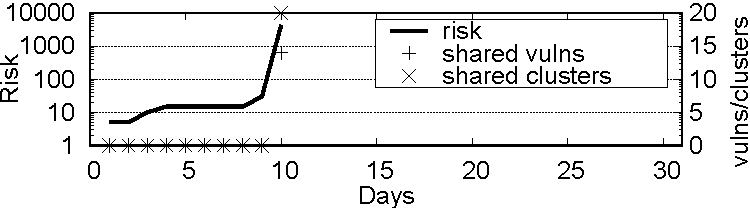
\includegraphics[width=0.5\columnwidth]{images/gnuplot/score/score_random_all.pdf}\label{fig:random_all}}
\hspace{0.5cm}
\subfigure[\system]{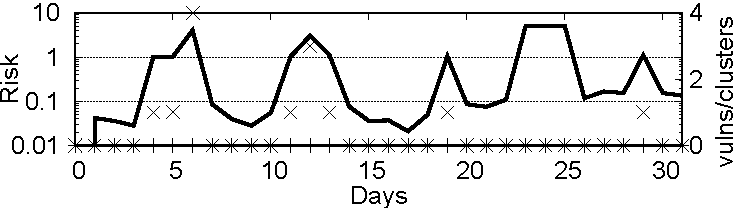
\includegraphics[width=0.5\columnwidth]{images/gnuplot/score/score_final_all.pdf}\label{fig:intel_all}}
\caption{Execution phase for Random and \system OS configuration strategies (log scale).}
\label{fig:run_all}
\end{figure*}

\textbf{Results:} As shown in Figure~\ref{fig:random_all}, \emph{Random} survives only for $10$ days. 
The number of shared clusters and vulnerabilities remains small for the first days. 
Then, there is a replica replacement that adds to the configuration an OS that has common vulnerabilities with the others. 
%Thus, enabling an adversary to compromise enough replicas in the system.

\system survives until the end of the experiment, as the risk is continually managed to keep the system safe. Figure~\ref{fig:intel_all} shows that shared clusters sometimes increase, at the same pace as the risk.
But then, the next reconfigurations are carried out with the goal of decreasing the risk. 
Notice that the risk value is always under $1$ for \system, and in the \emph{Random} is mostly above $10$.


\subsection{Diversity vs Attacks}

\begin{table}[t]
\begin{center}
{%\small%
\footnotesize
\begin{tabular}{ | p{0.96\columnwidth} | }\hline

\textbf{Samba:} 
\emph{On February 2, 2017, security researchers published details about a zero-day vulnerability in Server Message Block (SMB) of Windows, affecting several versions such as 8.1, 10, Server 2012 R2, and Server 2016. 
Could cause a \gls{dos} condition when a client accesses a malicious SMB.}\\
\textbf{CVES:} 
CVE-2017-0016
\\ \hline

\textbf{Wanna Cry:} 
\emph{On Friday, May 12, 2017, the world was alarmed to discover a widespread ransomware attack that hit organizations in more than 100 countries. Based on a vulnerability in Windows' SMB protocol (nicknamed EternalBlue), discovered by the NSA and leaked by Shadow Brokers.} \\
\textbf{CVES:} 
CVE-2017-0143, CVE-2017-0144, CVE-2017-0145, CVE-2017-0146, CVE-2017-0147, CVE-2017-0148 \\ \hline

\textbf{PowerShell:} 
\emph{Security feature bypass vulnerabilities in Device Guard that could allow an attacker to inject malicious code into a Windows PowerShell session.} \\
\textbf{CVES:}
CVE-2017-0219, CVE-2017-0173, CVE-2017-0215, CVE-2017-0216, CVE-2017-0218\\ \hline

\textbf{Stackclash:} 
\emph{In its 2017 malware forecast, SophosLabs warned that attackers would increasingly target Linux. The flaw, discovered by researchers at Qualys, is in the memory management of several operating systems and affects Linux, OpenBSD, NetBSD, FreeBSD and Solaris.}\\
\textbf{CVES:}
CVE-2017-1000365, CVE-2017-1000366, CVE-2017-1000367, CVE-2017-1000369, CVE-2017-1000370, CVE-2017-1000370, CVE-2017-1000371, CVE-2017-1000372, CVE-2017-1000373, CVE-2017-1000374, CVE-2017-1000375, CVE-2017-1000376, CVE-2017-1000379, CVE-2017-1083, CVE-2017-1084, CVE-2017-3629, CVE-2017-3630, CVE-2017-3631\\ \hline

\end{tabular}
}
\caption{Notable attacks during 2017.}
\label{tab:special_vulns}
\end{center}
\end{table}

This experiment evaluates the strategies when facing notable attacks/vulnerabilities that appeared in $2017$. 
Each attack potentially exploits several flaws, some of which affecting different \glspl{os}. 
The attacks were selected by searching the security news sites for high impact problems, most of them related to more than one CVE. 
As some of the \glspl{cve} include applications, we added more vulnerabilities to the database for this purpose.
Table~\ref{tab:special_vulns} lists the attacks and related \glspl{cve}: Samba,\footnote{https://www.secureworks.com/blog/attacking-windows-smb-zero-day-vulnerability} WannaCry,\footnote{https://securityintelligence.com/wannacry-ransomware-spreads-across-the-globe-makes-organizations-wanna-cry-about-microsoft-vulnerability/} Powershell,\footnote{http://blog.talosintelligence.com/2017/06/ms-tuesday.html} and Stackclash.\footnote{https://nakedsecurity.sophos.com/2017/06/20/stack-clash-linux-vulnerability-you-need-to-patch-now/}


Since some of these attacks might have been prepared months before the vulnerabilities are publicly disclosed, we augmented the execution phase to the full six months. 
As before, the strategies are analyzed over $5000$ runs.


\begin{figure}[t]
\begin{center}
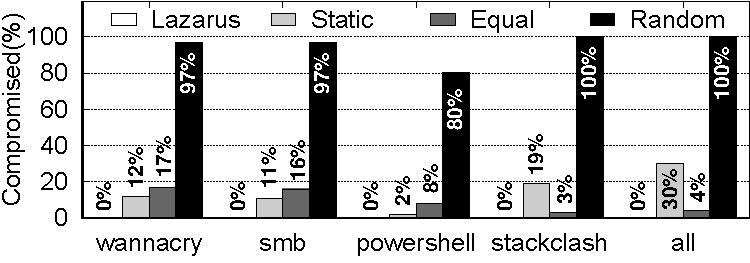
\includegraphics[width=\columnwidth]{images/gnuplot/special_vulns/execution-special.pdf}
\caption{Compromised runs with notable attacks.}
\label{fig:special_vulns}
\end{center}
\end{figure}

\textbf{Results:}
Figure~\ref{fig:special_vulns} shows the percentage of compromised runs for each attack and all attacks put together.
\system is clearly the best at handling the various scenarios, with no compromised executions.
\emph{Random} is the worse, as it does not use any criteria to select the OSes. 
Both \emph{Equal} and \emph{Static} may perform not so bad as they are static, i.e., the \glspl{os} selected by random chance might end up not being exploitable until the end of the run.


\section{Discussion}
\label{sec:discussionlazarus}
